\begin{center}\large\textbf{Readings: 15.1-15.5 700-732}\\
\normalsize \end{center}
\large \hlinewd{2pt}
~\\

Motivation - sometimes the variability of responses among experimental units is large, making detection of differences among treatment means $\mu_1,\mu_2,\ldots,\mu_t$ difficult.\\~\\
Using a Block design can help in this situation!\\

Example:  Suppose we are testing 2 drugs (A, B) on mice
\begin{itemize}
        \item{Response is mouse activity}
        \item{12 mice - We use a Completely Randomized Design (CRD)}
        \item{Find that treatment A increases activity significantly more than treatment B}
        \item{Fellow scientist notes that activity level may change based on the weight of the mice}
    \begin{itemize}
            \item{By random chance all of the treatment A mice are `small' and all the treatment B mice are `big'}
     \end{itemize}
\end{itemize}

Want to know if the drug was truly effective.  How can we account for the weight of the mice?  (ANCOVA is one option, but let's consider a different option).\\~\\
Should we use only small mice? only large mice?  Want to make inference to population as a whole.  Block design can remedy this!\\~\\

\newpage

Recall:
 \begin{itemize}
  \item{Blocking breaks the population up into subgroups (or blocks) \textbf{based on confounding variables that may have an effect on the response but are not of interest}}
        \begin{itemize}
            \item{No need to block on variables that don't effect the response}
        \end{itemize}
        \item{Experiment is run within each block then combined to make inference}
        \item{Permits inference to larger population while removing unwanted variability between units - allowing treatment effects to show up more clearly}
        \item{Technique reconciles two opposing aims of experimental design}
    \begin{enumerate}
        \item{Want our subjects to be homogeneous so subtle treatment differences can be seen}
        \item{Usually aim to make inferences relevant to a population of interest}
        \begin{itemize}
            \item{Our experimental units (subjects) must be representative of the population}
        \end{itemize}
    \end{enumerate}
\end{itemize}		

~\\~\\
\textbf{The Randomized Complete Block Design (RCBD)}
    \begin{itemize}
        \item{Experimenter creates Blocks of subjects (Block) - Goal:}
        \begin{itemize}
            \item{Try to make differences among blocks as large as possible}
            \item{Try to make differences within blocks as small as possible}
        \end{itemize}
        \item{Assume blocks are large enough to contain a complete replicate of the full set of treatments \textit{at least once} (Complete)}
        \item{Within each block, randomization is used to assign treatments to subjects (Randomized)}
        \item{Hence, Randomized Complete Block Design (RCBD)}
    \end{itemize}

Example:		
\begin{center}
\includegraphics[scale=0.43]{mice.png}
\end{center}

Randomized Complete Block Model (with fixed blocks, we assume our factor of interest is fixed)	
	$$Y_{ijk}=\mu+\beta_{i}+\tau_{j}+(\beta\tau)_{ij}+E_{ijk}$$~\\
Randomized Complete Block Model (with random blocks, we assume our factor of interest is fixed)			   
	$$Y_{ijk}=\mu+B_{i}+\tau_{j}+(B\tau)_{ij}+E_{ijk}$$~\\
    \begin{itemize}
    		\item{$\mu$ overall mean}
        \item{$i=1,...,b$ ($\#$ blocks)}
        \item{$\beta_{i}$ or $B_{i}$ represent block effects (assumed iid $\sim N(0,\sigma^2_{B})$, independent of other random effects if random blocks)}
        \item{$j=1,...,t$ ($\#$ treatments)}
        \item{$\tau_{j}$ represent treatment effects}
        \item{$(\beta\tau)_{ij}$ or $(B\tau)_{ij}$ represents the interaction between block and treatment (assumed iid $\sim N(0,\sigma^2_{B*Trt})$, independent of other random effects if random blocks)}
        \item{$k=1$ ($\#$ replications per block, assuming only 1)}
        \item{$E_{ijk}$ represent random errors (assumed iid $\sim N(0,\sigma^2)$, independent of other random effects)}
    \end{itemize}
~\\~\\
What might be an example of a fixed block?  a random block?\\~\\~\\~\\

\newpage

\begin{itemize}
        \item{If blocks fixed - statistical inferences apply only to the blocks used}
        \item{If blocks random - statistical inferences about treatment effects apply to the entire population}
        \item{Either way, analysis for the RCBD is the same!  As with CRD, can test for treatment effects by equating mean squares}\\
\end{itemize}
To test $H_{0}: \text{all } \tau_{j}=0$, can look at expected mean squares to find the appropriate test
	
\begin{center}Analysis of Variance Table for RCBD\end{center}
\scalebox{1}{
    \begin{tabular}{l|c|c|c}
    								& 					&Expected Mean Square				&Expected Mean Square\\
    Source					&df					&Fixed Block	&Random Block\\\hline
    Block						&b-1 				&$nt\phi_{B}^2+\sigma^2$ 		&$nt\sigma^2_{B}+n\sigma^2_{B*Trt}+\sigma^2$\\\hline
    Treatment				&t-1				&$nb\phi^{2}_{Trt}+\sigma^2$	&$nb\phi_{Trt}^2+n\sigma_{B*Trt}^2+\sigma^2$\\\hline
    Block*Treatment	&(b-1)(t-1)	&$n\phi_{B*Trt}^2+\sigma^2$	&$n\sigma^{2}_{B*Trt}+\sigma^{2}$\\\hline
    Error						&0					&$\sigma^2$									&$\sigma^2$
    \end{tabular}
    }
    \begin{itemize}
    	\item{$\phi^2$ terms are quadratic forms corresponding to the given fixed effect}
    	\item{$\sigma^2$ terms represent random effects}
    \end{itemize}
		
Notice:  Not possible to calculate a direct estimate of $\sigma^2$\\~\\
Recall: $\sigma^2$ is the error variance, or the variance of the population of measurements made under identical experimental conditions.\\~\\

In a RCB design, responses measured under identical experimental conditions are responses corresponding to a common block-treatment combination.  Consequently, $\sigma^2$ is the variance of the conceptual population of responses that can be observed for a given treatment within a given block.\\~\\

\newpage 

\textbf{What to do with fixed block?}\\
  \begin{center}Analysis of Variance Table for RCBD\end{center}    \scalebox{1}{
    \begin{tabular}{l|c|c|c}
    								& 					&Expected Mean Square				&Expected Mean Square\\
    Source					&df					&Fixed Block	&Random Block\\\hline
    Block						&b-1 				&$nt\phi_{B}^2+\sigma^2$ 		&$nt\sigma^2_{B}+n\sigma^2_{B*Trt}+\sigma^2$\\\hline
    Treatment				&t-1				&\hili{$nb\phi^{2}_{Trt}+\sigma^2$}	&$nb\phi_{Trt}^2+n\sigma_{B*Trt}^2+\sigma^2$\\\hline
    Block*Treatment	&(b-1)(t-1)	&\hili{$n\phi_{B*Trt}^2+\sigma^2$}	&$n\sigma^{2}_{B*Trt}+\sigma^{2}$\\\hline
    Error						&0					&\hili{$\sigma^2$}									&$\sigma^2$
    \end{tabular}
    }
    \begin{itemize}
   		\item{Fixed block, there is no ratio of mean squares to test the treatment}
			\item{If no Block*Treatment is reasonable ($\phi_{B*Trt}^{2}=0$) can use $$F_{Trt}=\frac{MS[Trt]}{MS[B*Trt]}$$ }    \\
		\end{itemize} 

\textbf{What to do with random block?}\\
    \begin{center}Analysis of Variance Table for RCBD\end{center}
    \scalebox{1}{
    \begin{tabular}{l|c|c|c}
    								& 					&Expected Mean Square				&Expected Mean Square\\
    Source					&df					&Fixed Block	&Random Block\\\hline
    Block						&b-1 				&$nt\phi_{B}^2+\sigma^2$ 		&$nt\sigma^2_{B}+n\sigma^2_{B*Trt}+\sigma^2$\\\hline
    Treatment				&t-1				&$nb\phi^{2}_{Trt}+\sigma^2$	&\hili{$nb\phi_{Trt}^2+n\sigma_{B*Trt}^2+\sigma^2$}\\\hline
    Block*Treatment	&(b-1)(t-1)	&$n\phi_{B*Trt}^2+\sigma^2$	&\hili{$n\sigma^{2}_{B*Trt}+\sigma^{2}$}\\\hline
    Error						&0					&$\sigma^2$									&$\sigma^2$
    \end{tabular}
    }
    \begin{itemize}
   		\item{For a random block, can use $F_{Trt}=\frac{MS[Trt]}{MS[B*Trt]}$ to test $H_{0}: \text{all } \tau_{j}=0$}
   		\item{In both cases $MS[B*Trt]$ is used as error term}\\
		\end{itemize} 
~\\
Recall: Interaction would imply treatment acts differently depending on block.
\begin{itemize}
    \item{If interaction truly exists:}
    \begin{itemize}
        \item{Only one complete replicate in each block, power of tests will be diluted}
        \item{If we have more than one complete replicate in each block, we can model interaction}
     \end{itemize}
     \item{If interaction does not exist:}
			\begin{itemize}
			  \item{More advantageous to include extra blocks rather than extra replications within blocks}
    \end{itemize}
	\end{itemize}
	
%last - Reason is that if blocking is being used to provide replication and the aim is to make inferences to the broader population from which the blocks are sampled, it is better to increase the number of blocks than to increase the number of units per treatment within a block.  The blocks have been constructed so as to maximize homogeneity among units within a block and at the same time (by random sampling) to represent the entire range of variability in the population.  The goal is to estimate the treatment effects under the entire range of conditions from which the blocks are sampled.  To obtain precise estimates of these treatment effects and powerful tests of them, it is necessary to have a sufficiently large sample of blocks.

\newpage

\textbf{Advantage of block design - Differences between treatment means don't involve blocks}\\
Assume we have a balanced design.  Denote the $j^{th}$ treatment mean by 
$$\hat{\mu}_{+j}=\mu+\bar{\beta}+\tau_{j}$$
We may be interested in a quantity such as 
$$\theta =\mu_{+2}-\mu_{+1}=\tau_{2}-\tau_{1}$$
Estimated by 
$$\hat{\theta} = \bar{y}_{+2}-\bar{y}_{+1}$$
Doesn't include the blocks!\\~\\

Making inference for means or differences of means:	\\	
\textbf{If blocks fixed:}
			\begin{itemize}
				\item{$\bar{y}_{.j}$ is interpreted as estimating $\mu+\bar{\beta}+\tau_{j}$}
				\item{Variance is $\sigma^{2}/b$}
				\item{Variance of $\hat{\theta}= \bar{y}_{+2}-\bar{y}_{+1}$ is $Var(\theta)=2\sigma^{2}/b$}
				\item{$\sigma^2$ is estimated by $MS(Block*Trt)$}
			\end{itemize}
Thus, when blocks are fixed, inference is equivalent to inference in the two-way ANOVA model using the interaction term as the error.\\~\\
\textbf{Blocks random:}
			\begin{itemize}
				\item{$\bar{y}_{.j}$ is an unbiased estimate of $\mu+\tau_{j}$}
				\item{Variance is $(\sigma_{B}^2+\sigma^2)/b$}
				\item{Degrees of freedom will need to be found using Satterthwaite's approximation!}
				\item{Variance of $\hat{\theta}= \bar{y}_{+2}-\bar{y}_{+1}$ is $Var(\theta)=2\sigma^{2}/b$}
				\item{$\sigma^2$ is estimated by $MS(Block*Trt)$}
			\end{itemize}
Thus, when blocks are random, inference for differences of treatment means don't involve blocks!\\~\\

We would of course want to make multiple comparison corrections for testing all pairwise differences of means.\\~\\

\newpage

\textbf{Example of RCBD:}
    \begin{itemize}
        \item{Scientist investigating Yield of Tomato plants - Has 5 different types of fertilizers}
        \item{Plants placed in pots on 3 benches in the greenhouse}
     		\item{5 pots can fit on each bench and there is a possible temperature gradient}
    \end{itemize}

\begin{center}
    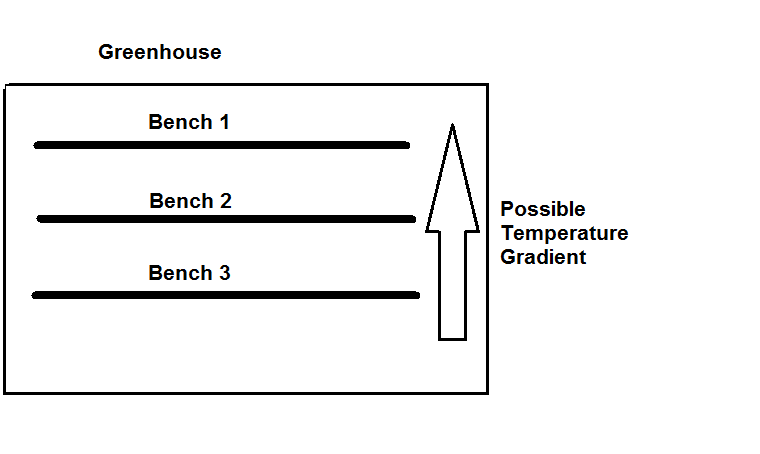
\includegraphics[scale=0.45]{layout1.png}
\end{center}

How can we set up our design to account for temperature gradient and reduce unexplained variation in response?\\~\\~\\~\\~\\
Blocks fixed or random here?\\~\\~\\~\\
Assumptions about interaction?\\~\\~\\~\\

\newpage

Analysis can be done in proc mixed (if replication, simply add random `Bench*Fertilizer' effect and use usual two-way mixed effects analysis):
\begin{small}
\begin{verbatim}
proc mixed method=type3 plots=all;
class Bench Fertilizer;
model Yield=Fertilizer/residual;
random Bench;
lsmeans Fertilizer/adjust=Tukey;
run;
\end{verbatim}
\end{small}

\begin{center}
\begin{tabular}{l|c|c|l|c|c}
    Source & DF  & MS & Error Term & Error DF & P-value\\\hline
    
Fertilizer     &      4      &  0.4164 &                   MS(Residual)  &     8&0.0017\\                       
Bench          &        2     &   0.0042     &                 MS(Residual)   &    8&0.8828\\
Residual      &      8   &   0.0338      &                   .            &              .&.
\end{tabular}
\end{center}
~\\
We can see we have a significant Fertilizer effect.  We don't care about the block effect significance.  Even if not significant we would leave this effect in!\\~\\
Remember, Residual here is really Fertilizer*Bench interaction.\\~\\

Differences of LSMeans\\
\begin{center}  
    \begin{tabular}{c|c|c|c}
  Fert  &   Fert  & Estimate &   Adj P\\\hline  
  1     &         2&     0.4133 &  0.1306\\
  1     &         3&     0.4267 &  0.1158\\  
  1     &         4&     0.5700&  0.0316\\  
  1     &         5&     1.0367 &  0.0008\\  
  2     &         3&   0.01333 &  1.0000\\  
  2     &         4&   0.1567 &  0.8293\\  
  2     &         5&     0.6233 &  0.0198\\  
  3     &         4&    0.1433  &  0.8679\\  
  3     &         5&     0.6100&  0.0222\\  
  4     &         5&    0.4667&  0.0805
\end{tabular}
\end{center}


Should always check model assumptions:
\begin{center}
		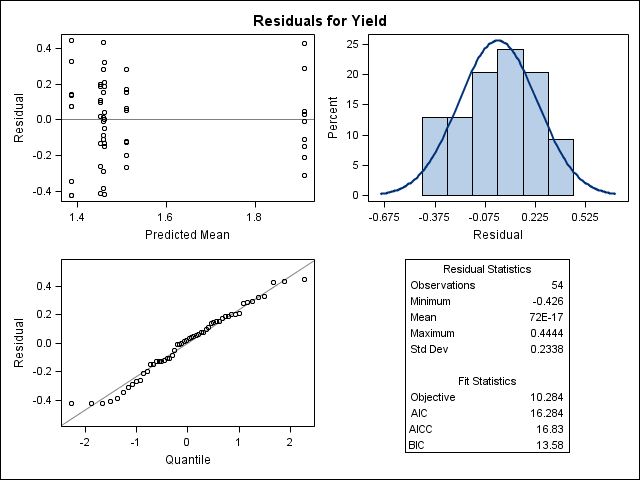
\includegraphics[scale=0.4]{ResidualPanel.png}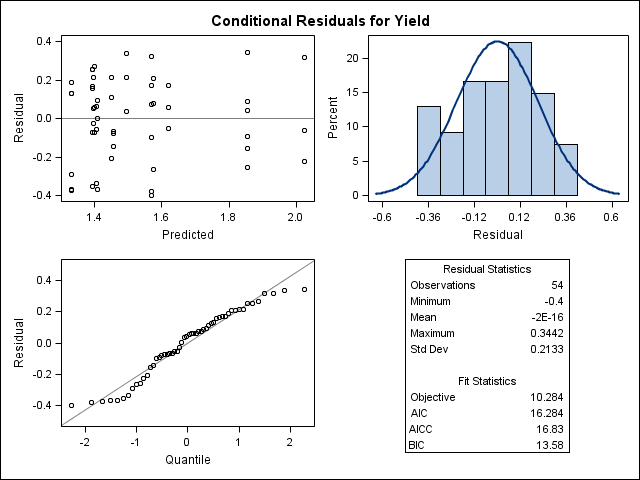
\includegraphics[scale=0.4]{ResidualPanel1.png}
\end{center}


\textbf{Relationship with ANCOVA - When to use the covariate with ANCOVA and when to use it to create blocks?}
    \begin{itemize}
        \item{If value not known until experiment underway or over (i.e. need to sacrifice animal to know) use ANCOVA}
        \item{If covariate nearly constant for groups use Blocking}
        \item{If not clear, guide based on correlation of covariate and response:}
        \begin{itemize}
        	\item{if correlation is less than 0.3 ignore}
        	\item{if correlation is between 0.3 and 0.6 use blocking}
        	\item{if correlation is greater than 0.6 use ANCOVA}
        \end{itemize}
        \item{Note: ANCOVA not very robust against failures of the ANOVA normality assumption - model must be correct}\\
    \end{itemize}
~\\
 \textbf{More Types of Block Designs}
    \begin{itemize}
        \item{Two blocking factors - Latin squares}\\~\\
        \item{For ordinal responses - Friedman Rank sum test}\\~\\
        \item{For binary response - Cochran's test}\\~\\
        \item{Restrictions on blocks - Incomplete block designs}\\~\\
    \end{itemize}

\textbf{Summary}
  \begin{itemize}
        \item{Randomized Complete Block Design is relatively simple, but powerful technique used to eliminate the effects of selected confounding variables when comparing treatments}
        \item{Allows for easier detection of treatment effects while having results apply to larger population}
        \item{Standard ANOVA assumptions plus Treatment and Block \textbf{do not} interact}
        \item{Very simple analysis and interpretation if balanced design}
\end{itemize}
